\documentclass[sigconf,review, anonymous]{acmart}
\acmConference[ESEC/FSE 2020]{The 28th ACM Joint European Software Engineering Conference and Symposium on the Foundations of Software Engineering}{8 - 13 November, 2020}{Sacramento, California, United States}
%
\usepackage{booktabs,algorithm,algorithmic,multirow,amsmath,xcolor,bm,makecell,balance} % For formal tables




\renewcommand{\algorithmicrequire}{\textbf{Input:}} 
\renewcommand{\algorithmicensure}{\textbf{Output:}}

% Copyright
%\setcopyright{none}
%\setcopyright{acmcopyright}
%\setcopyright{acmlicensed}
\setcopyright{rightsretained}
%\setcopyright{usgov}
%\setcopyright{usgovmixed}
%\setcopyright{cagov}
%\setcopyright{cagovmixed}
\newcommand\leaveout[1]{}


% DOI
\acmDOI{10.475/123_4}

% ISBN
\acmISBN{123-4567-24-567/08/06}

\acmYear{2020}
\copyrightyear{2020}

\acmPrice{15.00}


\begin{document}
\title{PROPER}
%\titlenote{Produces the permission block, and
%  copyright information}
\subtitle{a Tool for Analyzing Termination and Assertions for Probabilistic Programs}
%\subtitlenote{The full version of the author's guide is available as
%  \texttt{acmart.pdf} document}


\author{Ben Trovato}
%\authornote{Dr.~Trovato insisted his name be first.}
\orcid{1234-5678-9012}
\affiliation{%
  \institution{Institute for Clarity in Documentation}
  \streetaddress{P.O. Box 1212}
  \city{Dublin} 
  \state{Ohio} 
  \postcode{43017-6221}
}
\email{trovato@corporation.com}

\author{G.K.M. Tobin}
%\authornote{The secretary disavows any knowledge of this author's actions.}
\affiliation{%
  \institution{Institute for Clarity in Documentation}
  \streetaddress{P.O. Box 1212}
  \city{Dublin} 
  \state{Ohio} 
  \postcode{43017-6221}
}
\email{webmaster@marysville-ohio.com}

\author{Lars Th{\o}rv{\"a}ld}
%\authornote{This author is the one who did all the really hard work.}
\affiliation{%
  \institution{The Th{\o}rv{\"a}ld Group}
  \streetaddress{1 Th{\o}rv{\"a}ld Circle}
  \city{Hekla} 
  \country{Iceland}}
\email{larst@affiliation.org}

% The default list of authors is too long for headers}
\renewcommand{\shortauthors}{B. Trovato et al.}


\begin{abstract}
  Probabilistic programs combine probabilistic reasoning models with Turing complete programming languages, unify formal descriptions of calculation and uncertain knowledge, and can effectively deal with complex relational models and uncertain problems. This paper presents PROPER, a tool for analyzing termination and assertions for affine probabilistic programs. On one hand, it can help to analyze the termination property of affine probabilistic programs both qualitatively and quantitatively. It can check whether a probabilistic program terminates with probability $1$, estimate the upper bound of expected termination time, and calculate the number of steps after which the termination probability of the given probabilistic program decreases exponentially.  On the other hand, it can estimate the correct probability interval for a given assertion to hold, which helps to analyze the influence of uncertainty of variables on the results of probabilistic programs.
  %They can be effectively checked in polynomial time. PROPER supports  more than ten kinds of built-in probability distributions. 
  The effectiveness of PROPER is demonstrated through various affine probabilistic programs.
\end{abstract}

\leaveout{
%
% The code below should be generated by the tool at
% http://dl.acm.org/ccs.cfm
% Please copy and paste the code instead of the example below. 
%
\begin{CCSXML}
<ccs2012>
 <concept>
  <concept_id>10010520.10010553.10010562</concept_id>
  <concept_desc>Computer systems organization~Embedded systems</concept_desc>
  <concept_significance>500</concept_significance>
 </concept>
 <concept>
  <concept_id>10010520.10010575.10010755</concept_id>
  <concept_desc>Computer systems organization~Redundancy</concept_desc>
  <concept_significance>300</concept_significance>
 </concept>
 <concept>
  <concept_id>10010520.10010553.10010554</concept_id>
  <concept_desc>Computer systems organization~Robotics</concept_desc>
  <concept_significance>100</concept_significance>
 </concept>
 <concept>
  <concept_id>10003033.10003083.10003095</concept_id>
  <concept_desc>Networks~Network reliability</concept_desc>
  <concept_significance>100</concept_significance>
 </concept>
</ccs2012>  
\end{CCSXML}
}

\ccsdesc[500]{Software and its engineering~Software notatins and tools}

% We no longer use \terms command
%\terms{Theory}

\keywords{Probabilistic Programming, Program Verification, Termination, Ranking Supermartingale}


\maketitle


\section{Introduction}
There are a large number of uncertainty problems in the real world, which requires us to use prerequisite knowledge and deductive reasoning to predict the results, that is to say, to make decisions on nondeterministic problems through probability reasoning. Therefore, probabilistic programs are put forward for that purpose. Probabilistic programs are a kind of logic programs with probabilistic facts. They make probabilistic reasoning models easier to build and can estimate the possibilities of for certain events to occur.
Probabilistic programs have a wide range of applications in various fields such as business, military, scientific research and daily life. Probability is becoming more and more important in actual calculations, such as risk analysis, medical decision-making, differential privacy mechanisms, etc. The analysis of probabilistic programs has also received widespread attention in academia and industry. %Therefore, we need to learn the impact of probabilitisic variables on the program results, analyze and verify the properties of probabilistic grams, so as to ensure that the final results of the program have good reliability and stability.

In the current work we present presents PROPER, a verification tool for analyzing termination and assertions for affine probabilistic programs. It can automatically analyze whether an affine  probabilistic program conforms to a specification.
%(As shown in Figure \ref{syntaxy}).
It mainly includes two parts: one is to analyze the termination property of a given affine probabilistic program qualitatively and quantitatively; the other is to estimate the correct probability interval for a given assertion to hold.
More specifically, PROPER provides the following functionalities:
\begin{enumerate}
	\item Defining and parsing probabilistic programs. More than ten kinds of probability distributions are built in, which is convenient to be called to build probabilistic models.
    \item Reducing the termination analysis of a given program to a linear programming problem. We also consider the concentration results under the premise that the program is terminating.
	\item Reducing the estimation of a given assertion to a polyhedron solving problem. Note that we support probabilistic programs with infinitely many states.	
\end{enumerate}
The tool and the experimental data given in this paper are all available in the repository \url{https://github.com/Healing1219/PROPER}.

\section{Probabilistic Programs}
\begin{figure}[ht]
	\centering
	\begin{tabular}{rcl}
		\hline
		% after \\: \hline or \cline{col1-col2} \cline{col3-col4} ...
		program & $:=$ & typeSpecifier main\{$stmt^*$\} \\
		stmt & $:=$ & assign | condStmt | while \\
		assign & $:=$ & intAssign | realAssign \\
		condStmt & $:=$ & ifStmt | ifElseStmt\\
		while & $:=$ & while (test) $stmt^*$\\
		intAssign & $:=$ &  intVar = intConst | intVar $\sim$ intRandom\\
		realAssign & $:=$ & realVar = realConst | realVar $\sim$ realRandom\\
		intRandom & $:=$ & uniformInt(intConst, intConst)\\
		&  & | Bernoulli(intConst, intConst)\\
		&  & $\cdots$ \\
		realRandom & $:=$ & uniformReal(realConst, realConst)\\
		&  & | Gaussian(realConst, realConst)\\
		&  & $\cdots$ \\
		intExpr & $:=$ & intConst | intRandom | intExpr $\pm$ intExpr\\
		& & intConst* intExpr | intExpr / intConst\\
		realExpr & $:=$ & realConst | realRandom | realExpr $\pm$ realExpr\\
		& & realConst* realExpr | realExpr / realConst\\
		boolExpr& $:=$ & true | false | boolExpr $\wedge$ boolExpr \\
		& & intExpr relop intExpr | realExpr relop realExpr\\
		relop & $:=$ & <  |  > | $\geq$ | $\leq$ | ==\\
		\hline
	\end{tabular}
	\caption{Syntax specification of a probabilistic language}	\label{syntax}
\end{figure}
In order to analyze and verify probabilistic programs, we first need a probabilistic language sufficiently expressive and easy to understand. We follow \cite{Sankaranarayanan2013Static} to define a probabilistic language, whose syntax specification is shown in Figure~\ref{syntax}. The statements in the probabilistic language are similar to those in classic imperative languages, mainly composed of three types of statements: assignment, condition-branch (if-else) and loop statements (while). The main difference is that we now have a collection of random value generators(discrete distribution, Binomial distribution, Poisson distribution, Integer Uniform distribution, Real Uniform distribution, Exponential distribution, Gamma distribution, Beta distribution, Geometric distribution), which can be used to simulate different probability distributions. Variables are classified into two types: program variables and sampling variables. Program variables include integer, real, and boolean variables. Boolean variables are mainly used for condition and loop statements. Sampling variables are assigned with dynamically generated values when the program is running, which is subject to a continuous or discrete probability distribution.


We use control flow graphs (CFGs) to express the semantics of probabilistic programs. Formally, a CFG is a tuple in the form $(L,X,R,\mapsto,\bot)$, where:

\begin{itemize}
	\item $L$ is a finite set of labels $L=\{\ell_0,\ell_1,\dots,\ell_n\}$ used to represent control locations. Each statement in a program has a unique label. For example, $\ell_0$ usually indicates the starting location.
	%, $\ell$$_n$ indicates the last location.
	
	\item $X=\{x_0,\dots,x_n\}$ is a set of program variables and $R=\{r_1,\dots,r_m\}$ is a set of sampling variables.
	
	\item $\mapsto$ is a transition relation. Its element is in the form $(\ell,\alpha,\ell')$, representing one step of transition from control location $\ell$ to $\ell'$, by an update function $\alpha$: $\mathbb{R}^{|X\cup R|}\to \mathbb{R}^{|X|}$.
	
	\item $\bot$ is a sign of the exit of the program.
\end{itemize}


\begin{figure}[h]
	\centering
	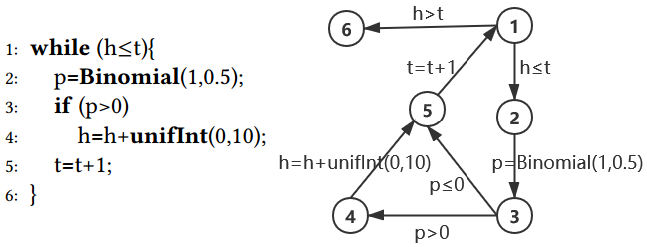
\includegraphics[scale=0.7]{img/example}
	\caption{A probabilistic program with its CFG}
	\label{example1}
\end{figure}

\paragraph{Example 1} In Figure~\ref{example1}, we show a probabilistic program on the left and its control flow graph on the right. In the program,  t is a program variable,  p and h are smapling variables. Here, two probability distributions are used: `Binomial(1,0.5)' represents a binomial distribution, which yields values 0 and 1 with equal chance; `unifInt(0,1)' represents an integer uniform distribution, which yields the integers between 0 and 10  with equal probability. The numbers 1-6 on the left are the program control locations, where 1 is the starting location and 6 is the terminal location. The probabilistic program simulates a scene of the tortoise hare race. The tortoise's initial position is t and the hare's initial position is h.  The tortoise  always moves at the speed of 1. With probability 0.5, the hare increases its speed by a random number between 0 and 10. The program terminates when the hare passes the tortoise.

\iffalse
\newcommand{\tabincell}[2]{\begin{tabular}{@{}#1@{}}#2\end{tabular}}
\begin{table}[htb]
	\caption{Specification of the inbuilt random value generators}
	\label{distribution}
	\begin{tabular}{lll}  
		\toprule   
		Name & Parameter & \makebox[4cm][c]{Density Function} \\  
		\midrule   
		R($\mathbb{X},\mathbb{P}$) & $\sum\limits_{n=1}^N p_n$=1 & $P(X=x_k)=p_k$\\  
		Binomial(n,p) & \tabincell{c}{0<p<1\\n$\geq$1} &$\tbinom{k}{n}p^k(1-p)^{n-k}, k=1,2,\dots$ \\  
		Poisson($\lambda$) & $\lambda$>0 &$\frac{\lambda^ke^{-\lambda}}{k!}$ \\   
		UnifInt(a,b) & a$\leq$b & 
		$\left\{
		\begin{array}{lr}
			\frac{1}{b-a} &, b>a \\
			1 & ,a=b\\
		\end{array}
		\right.$ \\
		UnifReal(a,b) & a<b & $\frac{1}{b-a}$ \\  
		Exponential($\theta$) & $\theta$>0 & $\frac{1}{\theta}e^{\frac{x}{\theta}}$ \\    
		Normal($\mu$,$\sigma^2$) &$\sigma$>0 &$\frac{1}{\sqrt{2\pi}\sigma}e^{-(x-\mu)^2/(2\sigma^2)}$ \\
		Gamma($\alpha$,$\beta$) & $\alpha, \beta$>0 & 
		$\frac{1}{\beta^\alpha\Gamma(\alpha)}x^{\alpha-1}e^{\frac{-x}{\beta}} , x>0 $  \\  
		Beta($\alpha$,$\beta$) & $\alpha, \beta$>0 & $\frac{\Gamma(\alpha+\beta)}{\Gamma(\alpha)\Gamma(\beta)}x^{\alpha-1}(1-x)^{\beta-1}$,0<x<1\\    
		Laplace(x|$\mu,\lambda$) & $\lambda>0$ &$\frac{1}{2\lambda}e^{\frac{|x-\mu|}{\lambda}}$ \\
		Geometric(p) & 0<p<1 & $(1-p)^{k-1}p, k=1,2,\dots$ \\     
		T(n) &n$\geq$1 &$\frac{\Gamma(\frac{n+1}{2})}{\sqrt{n\pi}\Gamma(\frac{n}{2})}(1+\frac{x^2}{n})^{-(n+1)/2}$ \\
		\bottomrule  
	\end{tabular}
\end{table}
\fi


\section{Termination Analysis}
Termination analysis is an important part of program verification.If the loop program is terminated for all initial values that can enter the loop, the program is said to be terminated.  Ensuring termination is a necessary condition for many properties of programs such as total correctness. Generally speaking, the termination of a program is undecideable~\cite{Turing1936On}, but for some subclass programs,its termination can be verified. In this paper, we prove the termination of the affine probabilistic programs by synthesizing ranking supermartingales~\cite{Chakarov2013Martingales}. PROPER implements Algorithm \ref{TA}~\cite{cha2015algorithmic,kris2016termination}to analyze probabilistic termination qualitatively and quantitatively. 
\begin{algorithm}[htb]  
	\caption{Termination Analysis.}  
	\label{TA}  
	\begin{algorithmic}[1]  
		\REQUIRE 
		Program P; 
		\ENSURE  
		Judge whether the program is terminating, isT;\\
		The probability to terminate afer N steps decreases exponentially, N.
		\STATE Set template $g(\ell,\boldsymbol{x})$ with a natural number as the maximal degree. Each location has the common template with unique coefficient. If $\ell_{\bot}$, the template $g(\ell,\boldsymbol{x})$=K.
		\STATE Traverse the programs parse tree \\
		2.1: Collect the invariant I[] for each location.\\
		2.2: Calculate the pre-expectation for each location.\\
		\quad \quad case "assignment statement" :\\
		\quad \quad \quad \quad $pre(\ell,\boldsymbol{x})= \mathbb{E}(g(\ell',\alpha,\boldsymbol{x})$.\\
		\quad \quad case "condition(if-else) or loop(while) statement" :\\
		\quad \quad \quad \quad $pre(\ell,\boldsymbol{x})=g(\ell',\boldsymbol{x})$.\\
		\quad \quad case "terminal statement" :\\
		\quad \quad \quad \quad $pre(\ell,\boldsymbol{x})=g(\ell,\boldsymbol{x})=K$.
		\STATE By the concept of half-space, $H=g(\ell,\boldsymbol{x})-pre(\ell,\boldsymbol{x})-\epsilon$, where $\epsilon >0$ and $K \leq -\epsilon$
		\STATE Pattern extraction. By Handelman's Theorem, $H'=\sum\limits_{i=1}^{d} a_i\cdot \mu_i$, where $\mu_i \in \mu$, $\mu=\{\prod\limits_{i=1}^{n} I_i | n\in\mathbb{N}_0 and I_1,\dots,I_n \in I\}$ and $a_i$ is a non-negative real number.
		\STATE Solve linear programming. H and H' are corrsponding coefficient relations. If solvable, the program P can be terminating, otherwise return.
		\STATE Calculate the upper bound of expected termination time according to $EP(P)\leq UB(P):=\frac{g(\ell_0,x_0)-K}{\epsilon}$
		\STATE Calculate the difference interval $[a,b]$ satisfying the condition $a\leq g(\ell',\boldsymbol{x})-g(\ell,f(\boldsymbol{x},\boldsymbol{r}))\leq b$
		\STATE Obtain N, according to $\mathbb{P}(\bm{T_p} > N) \leq e^{-\frac{2(\epsilon(N-1)-g(\ell_0,x_0))^2}{(N-1)(b-a)^2}}$
	\end{algorithmic}  
\end{algorithm}  


\paragraph{Qualitative analysis} It mainly analyzes whether the probabilistic programs will terminate with probability $1$ (almost sure termination). The specific idea is to calculate the martingale of each location and the value of location $\ell$' minus the value of location $\ell$ is $\epsilon$, where $\epsilon$ is greater than $0$. Refer to Algorithm \ref{TA} steps 1 to 5. The polynomial ranking supermartingale(RSM) is a collection of functions at each label, represented by the template $g(\ell,\cdot)$. Each function is non-negative at non-terminal program position. The invariants and pre-expectation are calculated by traversing the program parse tree. The pre-expectation~\cite{Chakarov2013Martingales} is about the expression over the variables across a transition $\mapsto$. Then, through steps 3 and 4, H and H' can be known. According to Handelman's theorem~\cite{Handelman1988Representing}, we know that the coefficients of H and H' match exactly. So we obtain a linear programming problem.  For the sake of simplicity, in PROPER, we take the maximal degree of the template as $2$, that is, the template $g(\ell,\cdot)$ is a quadratic equation. In addition, $\epsilon$ is taken as $1$ and K as $-1$ for our tool PROPER. Below we show the RSM of Example 1 in Table \ref{RSM}. 

\begin{table}[htb]
	\centering
	\caption{The RSM for Example 1}
	\label{RSM}
	\begin{tabular}{|c|c|c|}
		\hline
		Lable& Invariant & The RSM g \\ \hline
		1 & $h\leq t+9$ &$3\cdot t-3\cdot h+27$ \\ \hline
		2 & $h\leq t$ &$3\cdot t-3\cdot h+26$ \\ \hline
		3 & $h\leq t$  &$3\cdot t-3\cdot h-14\cdot p+32$ \\ \hline
		4 & $h\leq t\land p=1$ &$3\cdot t-3\cdot h+17$ \\ \hline
		5 & $h\leq t+10$&$3\cdot t-3\cdot h+31$ \\ \hline
		6 & $t<h$ &$-1$ \\ \hline
	\end{tabular}
\end{table}

The "Label" column lists control locations of the program. The "Invariant" column gives the logical formula that the reachable value on each label satisfies when the program is executed from the starting location. The "The RSM g" column denotes the ranking supermartingale on the label. The expected value of the RSM decreases by at least a positive amount $\epsilon$ after each execution of a statement. For example, 
when going from  from label 1 to label 2, the expected value of the supermartingale decreases by 1. Similarly  in the step from label 2 to label 3,  the condition is met because $\mathbb{E}(Binomial(1,0.5))=0.5$.
%meet the above condition. Similarly, from label 3 to label 4, $g(\ell_3,h,t,\mathbb{E}(Binomial(1,0.5)))-g(\ell_4,h,t,1)=1$; from lable 3 to label 5, $g(\ell_3,h,t,0)-g(\ell_5,h,t,0)=1$; from label 4 to label 5,  $g(\ell_4,h,t,0)-g(\ell_5,\mathbb{E}_r(h+r),t,0)=1$, where $r=unifInt(0,10)$ and from label 5 to label 1, $g(\ell_5,h,t,p) -g(\ell_1,h,t+1,p)=1$, they are also satisfied. At program exit, we have from the invariant $h\leq t+9$ that $g(\ell_1,h,t,0)-g(\ell_6,h,t,p)\geq 1$ which satisfy the condition.

\paragraph{Quantitative analysis} We aim to estimate the upper bound of expected termination time and calculate the boundary $N$, so that the probabilistic program concentrates on termination before $N$ steps. 
We focus on the approximation of the expected termination time, as given in steps 6 to 8 in Algorithm \ref{TA}. According to the previous steps, we can find the coefficients of the polynomial template RSM. The existence of an RSM ensures a finite upper bound on the expected termination time. If we know the initial values of variables, we can see that the value at the first location is $g(\ell, x_0)$, the value is $K$ at the terminated location $\ell_\bot$ and the difference between two consecutive locations is $\epsilon$.  Therefore, when program $P$ is almost surely terminating, we can get the upper bound on termination time for the given initial condition: $ET(P) \leq UB(P) = \frac{g(\ell, x_0)-K}{\epsilon}$. 
Then we focus on concentration problem, that is, the probability of termination after $N$ steps shows an exponential decrement. Exponential sum is one of the most commonly used specific function families in nonlinear approximation theory. Our main idea is based on martingale inequality of Azuma's Inequality~\cite{Azuma1967}, Hoeffding's Inequality~\cite{Hoeffding1963,McDiarmid1998Concentration}  and Bernstein's Inequality~\cite{Bennett1962,McDiarmid1998Concentration}. In probability theory, the Azuma's inequality gives a concentration result for the values of martingales that have bounded differences. Hoeffding's Inequality is a special case of Azuma's Inequality. It proposes an upper bound on the probability that the sum of random variables deviates from its expected value. Bernstein's Inequality is a generalization of Hoeffding. It can handle not only independent variables but also weak independent variables. By \cite{cha2015algorithmic}, we know that if $\epsilon(N-1) > g(\ell_0,\boldsymbol{x_0})$, the inequality $\mathbb{P}(\bm{T_p} > N)\leq e^{-\frac{2((N-1)-g(\ell_0,x_0))^2}{(N-1)(b-a)^2}}$ holds. 
%Given the exponent, we can obtain the result of $N$.
Consider again Example 1 with the initial values t=30 and h=5. We have  $ET(P) \leq \frac{3\cdot 30-3\cdot 5+27-K}{\epsilon}=103$, where $K$ and $\epsilon$ are set to be -1 and 1, respectively. Thedifference interval exists, which is [-28,14]. Suppose we make the query $\mathbb{P}(\bm{T_p} > N)\leq 10^{-3}$, the number N can be computed to be 6296  approximately.

\begin{figure}[h]
	\centering
	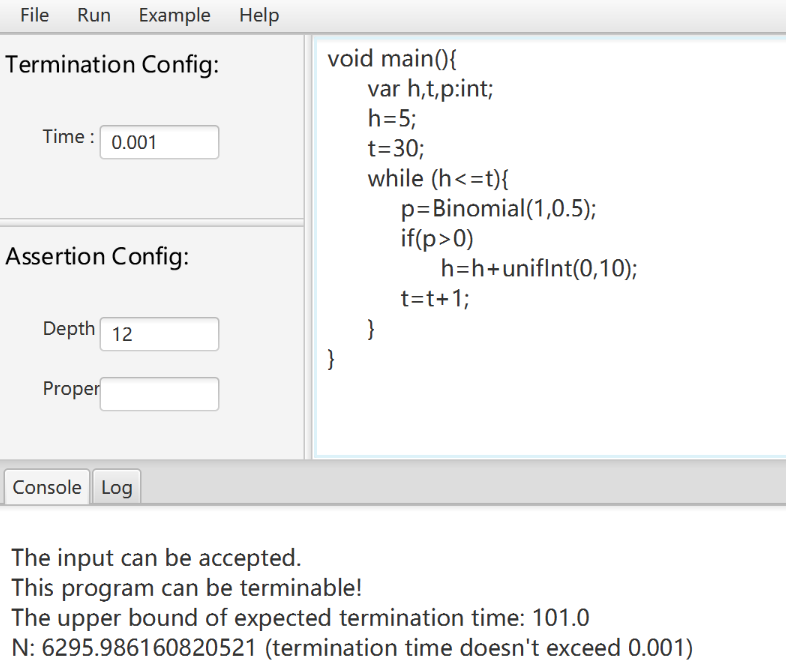
\includegraphics[scale=0.6]{img/interface}
	\caption{PROPER User Interface}
	\label{interface}
\end{figure}

The user interface is shown in the Figure \ref{interface}. The concentration termination time can be set on the upper left of the interface and the probabilistic programs can be written on the right. Alternatively, a probabilistic program  can be imported from an external file. 
Then by clicking ``Termination Analysis" in the ``Run" drop-down menu, we start the analysis process. The analysis results are displayed in the console. 


\section{Estimating the probabilities of assertions}
The goal of this section is to estimate the probability that a given assertion is correct at the exit of the program. The specific algorithm can refer to~\cite{Sankaranarayanan2013Static}. There are two main steps.

\begin{table*}[htb]
	\caption{Experimental results: termination analysis}  
	\label{TerminationResult} 
	\begin{center}  
		\begin{tabular}{|l|l|l|l|l|}  
			\hline  	
			Example & $x_0$ & g($\ell_0,x_0$) & UB(P) & N (time$\leq$0.01 sec)\\ \hline  	
			Simple & $x=100$  & $6x$ & 601 & 1474.82 \\ \hline  		
			NestedLoop & $x=1, m=2$ & $1040\cdot m-1040\cdot x+208$ & 1249 & 158141.27 \\  \hline  
			Award & bonus=0 & -4.0$\cdot$bonus+440& 441 &4522.28 \\  \hline  
			RandomWalk & $position=0$ & -20$\cdot$position+120 & 121 & 4695.66 \\  \hline  
			Gambler& $money=3$ & 400$\cdot$money+400& 1601 & 1506477.30 \\ \hline  		 
			Gambler2 & $money=10$ & 45.454545$\cdot$money+454.545455 & 910.09 & 1297006.47 \\  \hline  
			Bitcoin mining & $coin=10$ & 5.317601$\cdot$coin & 54.18 & 6.387839E7 \\  \hline 
			Tortoise-Hare & $h=5$, $t=30$ & 3$\cdot$t-3$\cdot$h+27 & 103 & 4264.27 \\  \hline  
		\end{tabular}  
	\end{center}  
\end{table*}

The first step is to generate a sufficient and appropriate path set $S$ with high confidence coverage. Using symbolic execution~\cite{Geldenhuys2012symbolic}, the finite set $S=\{s_1,\dots,s_i,\dots,s_n\}$ contains distinct paths that are terminating, that is, we have the transition sequences $s_i: \ell_0 \to \dots \to \ell_k \to \dots \to \ell_{\bot}$.The second step is to estimate the probability of a given assertion $\varphi$. For the path set S collected above, we can analyze each path in turn, then estimate the path probability and eventually the assertion probability. Since the calculation of the accurate probabilities is closely related to the volume of $n$-dimensional convex polyhedron, when the dimension increases, the calculation becomes very difficult and the time complexity is high~\cite{Arora1998Proof}. Usually, the computation may fail due to the calculation or insufficient memory. On the premise of weighing the efficiency and accuracy of calculation, we focus on calculating the probability interval of a given assertion rather than the estimated value.

\section{Experimental Results}
In this section, we present some experimental results of analyzing probabilistic programs using PROPER. More details can be found at GitHub.


We have written some simple but classical probabilistic programs with `while' loops. In Table~\ref{TerminationResult}, we display the experimental results about termination analysis, where $x_0$ means the initial value of each variable, $g(\ell_0,x_0)$ is the polynomial ranking supermartingale about the starting location, $UB(P)$ is the upper bound of expected termination time and $N$ is the bound that the probability of termination after $N$ steps shows an exponential decrement (we set the exponent to  $0.01$).


\begin{table}[htb]
	\caption{Experimental results: estimating the probability interval of assertions}
	\label{AssertionsResults} 
	\begin{tabular}{c |c |c |c }
		\hline  
		Ex. & Assertion &  $c$ & Bounds \\ \hline
		\iffalse
		\multirow{2}{*}{carton}
		& count$\geq$5 & 0.9485 & [0.948540, 1] \\ \cline{2-4}
		& count$\geq$10 & 0.9539, & [0.000639, 0.046711] \\ \cline{2-4}
		& count$\leq$7 & 0.9549 & [0.918762, 0.963832] \\ \cline{2-4}
		& totalWeight$\geq$5.5 & 0.9386 & [0.382145, 0.453010] \\ \cline{2-4}
		& totalWeight$\geq$6 & 0.9428 & [0.246186, 0.342997]  \\ \hline
		\fi
		\multirow{2}{*}{herman}
		& count$\geq$1 & 0.9561 & [0.581128, 0.625000] \\ \cline{2-4}
		& count$\geq$20 & 0.9701 & [0.000000, 0.029876]  \\ \hline
		\multirow{3}{*}{\makecell[c]{framin\\gham}}
		& points$\geq$10 & 0.9636 & [0.137343, 0.173695] \\ \cline{2-4}
		& pointsErr-points$\geq$5 & 0.9365 & [0.778149, 0.849318]  \\ \cline{2-4}
		& points-pointsErr$\geq$5 & 0.9326 & [0.177619, 0.246763]  \\ \hline
		\multirow{5}{*}{\makecell[c]{sum-\\three}}
		& $x>5 \ \&\& \ y>0$ & 0.9886 & [0.150535, 0.163590]  \\ \cline{2-4}
		&  \makecell[c]{$x>0 \ \&\&\ y>0$ \\ $\&\& \ z>0$} & 0.9886 & [0.125582, 0.137293] \\ \cline{2-4}
		& $x+y>z+10$ & 0.9886 & [0.447672, 0.470723] \\ \cline{2-4}
		& $x+y+z>8$ & 0.9886 & [0.454482, 0.475890] \\ \cline{2-4}
		& $x+y+z>100$ & 0.9886 & [0.012422, 0.025870]  \\ \hline
		\multirow{2}{*}{ckd-epi}
		& $f -f_1\geq0.1$ & 0.9252 & [0.351632, 0.426397] \\ \cline{2-4}
		& $f_1 -f\geq0.1$ & 0.9261 & [0.387275, 0.461157]  \\ \hline
		
	\end{tabular}  
\end{table}

The result of estimating the probability interval of assertions is consistent with paper~\cite{Sankaranarayanan2013Static}, as shown in Table~\ref{AssertionsResults}. A little difference lies in the syntax rules of assertions. We support logical operator conjunction ``\&\&" in PROPER. It can analyze situations where two or more conditions are met at the same time. In the table, an assertion is a boolean expression; $c$ is the lower bound of path coverage; the column headed by Bounds gives the upper and lower bounds of the given assertion.%Due to layout restrictions, some values are not presented in the table, such as the total number of execution paths and unique paths.

\section{Related Tools}
Sofware tools for the analysis of probabilistic programs has not yet received much attention. 
As far as we know, the only existing tools are ProbFuzz~\cite{DBLP:conf/sigsoft/DuttaLHM18}, PSense~\cite{DBLP:conf/atva/HuangWM18} and PSI~\cite{DBLP:conf/cav/GehrMV16}.
PSI is a symbolic inference tool that approximates the probability density function represented by a probabilistic program. 
PSense is an automated verification tool that generates tight upper bounds for the sensitivity of probabilistic programs over initial inputs.
ProbFuzz is a tool for testing probabilistic programs. 
Both the aforementioned tools do not consider termination analysis of probabilistic programs. 
For example, ProbFuzz focuses on testing rather than verification of probabilistic programs, 
PSI considers only inference and PSense solves sensitivity instead. 
Moreover, PSI/PSense requires that the input probabilistic while loop has a bounded number of loop iterations, while we can handle probabilistic loops with an unbounded number of loop iterations.

\section{Conclusions and Future Work}
Uncertainty exists in many software systems, including data analysis, stochastic algorithms and Monte Carlo simulation~\cite{HASTINGS1970Monte}. We have designed PROPER  to provide convenience and support for analyzing probabilistic programs.
PROPER is helpful to perform qualitative and quantitative analysis on the termination of probabilistic programs. It can also collect path sets with high confidence coverage and compute  probability interval for assertions to hold in probabilistic programs.


However, we have only solved some aspects of the complex problem of probabilistic program analysis and verification. There are still many ways to improve the tool.
\begin{enumerate}
	\item Currently, PROPER only deals with linear programs. That is, it cannot handle variable multiplication, division and exponents, etc., regardless of the termination analysis or the estimation of assertion probability interval.
	\item Non-deterministic probabilistic programs  are also not supported. PROPER requires the the behavior of the input program to be fully probabilistic, and there is no non-deterministic transitions. 
	\item In the future, we hope to find a better way to compute more accurate termination time and probability interval under the premise of ensuring high efficiency~\cite{Hermanns2013Probabilistic}. 
\end{enumerate}




%\appendix
%Appendix A
% \section{Headings in Appendices}

% \subsection{Introduction}
% \subsection{The Body of the Paper}
% \subsubsection{Type Changes and  Special Characters}
% \subsubsection{Math Equations}
% \paragraph{Inline (In-text) Equations}
% \paragraph{Display Equations}
% \subsubsection{Citations}
% \subsubsection{Tables}
% \subsubsection{Figures}
% \subsubsection{Theorem-like Constructs}
% \subsubsection*{A Caveat for the \TeX\ Expert}
% \subsection{Conclusions}%

% This next section command marks the start of
% Appendix B, and does not continue the present hierarchy

%\begin{acks}


%\end{acks}


\newpage
\balance
\bibliographystyle{ACM-Reference-Format}
\bibliography{sigproc} 

\end{document}
